\chapter{Plataforma de desarrollo}
\label{cap:capitulo3}

\begin{flushright}
\begin{minipage}[]{10cm}
\emph{Quizás algún fragmento de libro inspirador...}\\
\end{minipage}\\

Autor, \textit{Título}\\
\end{flushright}

\vspace{1cm}

Escribe aquí un párrafo explicando brevemente lo que vas a contar en este capítulo. En este capítulo, explica qué has usado a nivel hardware y software para poder desarrollar tu trabajo: librerías, sistemas operativos, plataformas, entornos de desarrollo, etc.

\section{Raspberry Pi 4 Model B}

La Raspberry Pi 4 Model B (Figura \ref{fig:raspberry2}) es la plataforma hardware de bajo coste escogida para este proyecto. Debido a la gran comunidad de desarrolladores y usuarios que posee, además de las especificaciones ofrecidas (Cuadro \ref{cuadro:especificaciones_rpi4}) por su escaso precio (65,44 \euro\footnote{Distribuidor oficial de Raspberry: \url{https://www.kubii.es/40-raspberry-pi-3-2-b}}), es la plataforma más usada por la mayoría del público.\\

\begin{figure} [h!]
  \begin{center}
    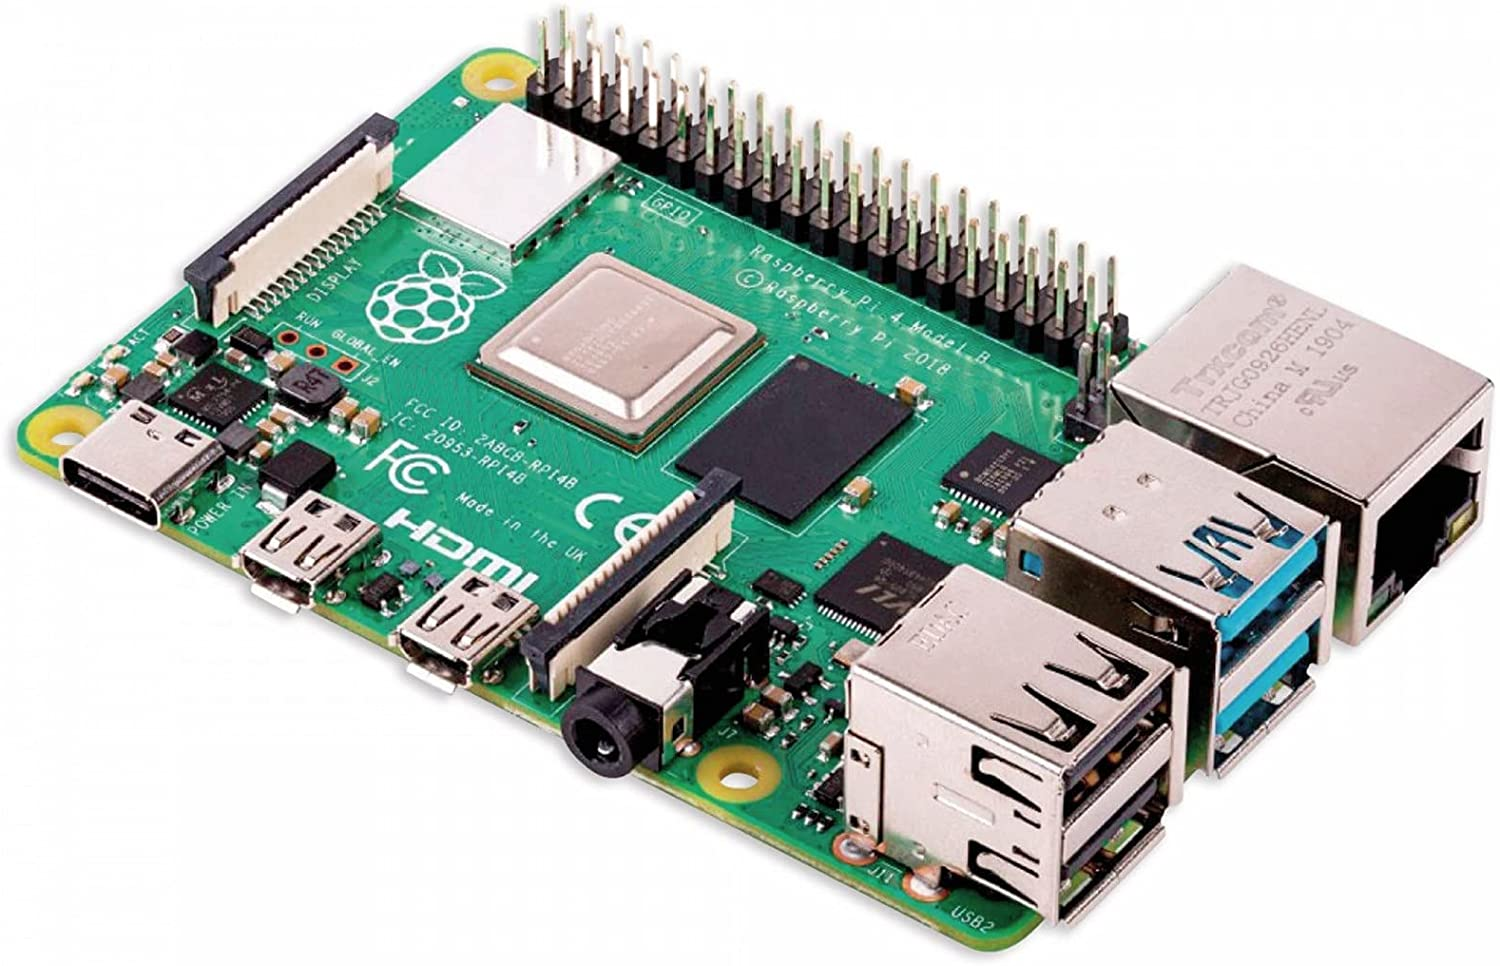
\includegraphics[width=9cm]{figs/raspberry.jpg}
  \end{center}
  \caption{Raspberry Pi 4b.}
  \label{fig:raspberry2}
\end{figure}

Sus características más atractivas ---entre otras--- son su bajo consumo energético, su pequeño tamaño y por lo tanto mínimo peso, su alta conectividad y puertos (red WIFI, Bluetooth, Ethernet, USB2 y USB3, HDMI, etc.) y la gran fluidez que posee su sistema operativo (Sección \ref{sec:raspberry_pi_os}). Todo esto la convierte en una auténtica joya y son cada vez más usuarios los que la utilizan en diversos proyectos. Podemos encontrarla ---por ejemplo--- como centro doméstico inteligente para controlar la domótica de una casa o incluso en sectores más profesionales formando parte de la arquitectura de algunos robots. Esto último es lo más interesante, para nosotros, dentro de los múltiples usos que tiene una Raspberry.\\

\begin{table}[H]
\begin{center}
\begin{tabular}{|>{\centering\arraybackslash}m{3cm} | >{\arraybackslash}m{6cm} |}
     \hline
     Procesador & Broadcom BCM2711 (4 núcleos Cortex-A72 (ARM v8), 64-bit, 1.5Ghz) \\ \hline
     Tarjeta gráfica & Broadcom VideoCore VI (integrada en el procesador) \\ \hline
     Memoria RAM & 4 GB LPDDR4-3200 SDRAM \\ \hline
     \multirow{3}{*}{Conexión}& WIFI 2.4 GHz y 5 GHz\\
     & Bluetooth 5.0/BLE\\
     & Gigabit Ethernet \\ \hline
     \multirow{5}{*}{Puertos}& 2 x micro-HDMI (4K 60 Hz)\\
     & MIPI Display Serial Interface \\
     & MIPI Camera Serial Interface \\
     & Jack Audio/Video \\
     & Slot para micro-SD \\ \hline
     \multirow{2}{*}{Alimentación} & 5V por USB-C (3A mínimo) \\
     & 5V por GPIO (3A mínimo) \\ 
     \hline
 \end{tabular}
\caption{Especificaciones técnicas de la Raspberry Pi 4 Model B.}
\label{cuadro:especificaciones_rpi4}
\end{center}
\end{table}

Gran parte de los robots son de tamaño reducido y no tienen el espacio suficiente como para acoplar una gran estación de procesamiento, por lo tanto en esos casos es muy común usar algún modelo de Raspberry como unidad central. Incluso en robots grandes se suelen utilizar también para realizar el control de zonas concretas, por ejemplo de los ojos de un humanoide. Por lo tanto, nuestro sistema de detección de emociones corriendo en la Raspberry Pi 4 Model B puede servir de gran ayuda a la hora de construir uno de estos robots comentados anteriormente que sólo tienen la capacidad de albergar una placa de tamaño reducido, o que simplemente los desarrolladores de dicho robot quieren ahorrar dinero en costes.

\subsection{Raspberry Pi OS}
\label{sec:raspberry_pi_os}

Raspberry Pi OS es el sistema operativo oficial para Raspberry. Es un sistema operativo gratuito basado en Debian optimizado específicamente para el hardware de la Raspberry Pi, por lo tanto es el que mayor rendimiento nos ofrecerá frente a otros como Ubuntu (que también puede ser instalado). Además, está en constante desarrollo y continuamente se está mejorando su estabilidad y funcionalidad. Es por todo ello que será el sistema operativo elegido en nuestro proyecto, sobre todo por su alto rendimiento (algo esencial para impulsar el desempeño de nuestro sistema de detección de emociones).\\

La versión de Raspberry Pi OS escogida ha sido Raspberry Pi OS Legacy (Cuadro \ref{cuadro:especificaciones_rpios}). Se ha elegido dicha versión porque, de todas las disponibles, ha sido la única en la que se ha conseguido instalar una versión de ROS/ROS2 (en concreto, ROS Noetic). Además, aunque las versiones de Raspberry Pi OS de 64-bit ofrecían más rendimiento, todavía no estaban maduras y no ofrecían total compatibilidad con todas las librerías usadas en el presente trabajo.

\begin{table}[H]
\begin{center}
\begin{tabular}{|>{\centering\arraybackslash}m{4cm} | >{\arraybackslash}m{4cm} |}
     \hline
     Fecha de lanzamiento & 4 de Abril de 2022 \\ \hline
     Sistema & 32-bit \\ \hline
     Versión del Kernel & 5.10 \\ \hline
     Versión de Debian & 10 (buster) \\ \hline
 \end{tabular}
\caption{Especificaciones de Raspberry Pi OS Legacy.}
\label{cuadro:especificaciones_rpios}
\end{center}
\end{table}

\subsection{Raspberry Pi Camera Module V2.1}

